\documentclass[10pt]{beamer}

\usetheme{metropolis}
\definecolor{WiLabRed}{RGB}{197,18,48}
\setbeamercolor{frametitle}{fg=white,bg=WiLabRed}
\setbeamercolor{progress bar}{fg=WiLabRed!90}
\setbeamercolor{title separator}{fg=WiLabRed!90}
\setbeamercolor{progress bar in section page}{fg=WiLabRed!90}
\setbeamercolor{background canvas}{bg=white}
\setbeamercolor{alerted text}{fg=WiLabRed!90}

\usepackage{appendixnumberbeamer}

\usepackage{booktabs}
\usepackage[scale=2]{ccicons}

\usepackage{pgfplots}
\usepgfplotslibrary{dateplot}

\usepackage{xspace}
\newcommand{\themename}{\textbf{\textsc{metropolis}}\xspace}

\usepackage{marvosym}
%\usepackage{subfig}
\usepackage{graphicx}\graphicspath{{images/}}
\usepackage{subcaption}
\usepackage[framed]{mcode}
\usepackage{listings}

\title{Lecture 01: Software Defined Radio Primer}
\subtitle{\textit{Software Defined Radio for Engineers} (Collins~\textit{et al.}), \textsection{1.2}}
\date{}
\author{\textbf{Alexander M. Wyglinski, Ph.D.}}
\institute{ \vspace*{1in}\hfill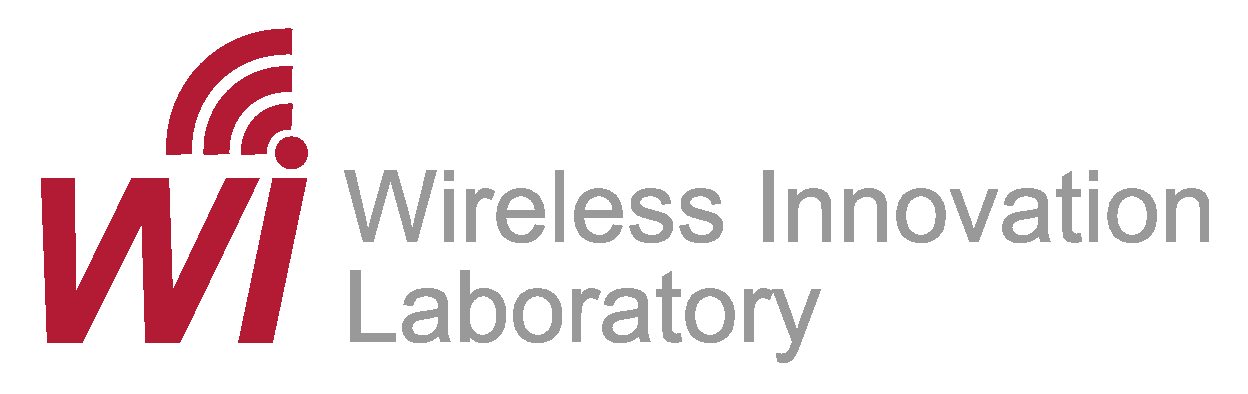
\includegraphics[height=1.125cm]{wilab_logo-A70916.eps} \qquad 
\includegraphics[height=1.125cm]{WPI_Inst_Prim_FulClr.eps}}
% \titlegraphic{\hfill\includegraphics[height=1.5cm]{logo.pdf}}

% Foot for all slides
\setbeamertemplate{frame footer}{\tiny \copyright~2018 by Alexander Wyglinski. This work is licensed under the Creative Commons Attribution-ShareAlike 4.0 International License. To view a copy of this license, visit http://creativecommons.org/licenses/by-sa/4.0/.}

\begin{document}

%\captionsetup[subfigure]{labelformat=empty}

%%%%%%%%%%%%%%%%%%%%%%%%%%%%%%%%%%%%%%%%%%%%%%%%%%%%%%%%%%

\maketitle




%%%%%%%%%%%%%%%%%%%%%%%%%%%%%%%%%%%%%%%%%%%%%%%%%%%%%%%%%%

\begin{frame}[fragile]{What Is A Communication System?}


\centering
Information Source\\
$\downarrow$\\
Conversion to EM Signal\\
$\downarrow$\\
Transmission Medium\\
$\downarrow$\\
Conversion from EM Signal\\
$\downarrow$\\
Information Sink

\end{frame}



%%%%%%%%%%%%%%%%%%%%%%%%%%%%%%%%%%%%%%%%%%%%%%%%%%%%%%%%%%

\begin{frame}[fragile]{Course Objectives}

What we are focusing on in this course:
\begin{itemize}
 \item Conduct various performance analyses of digital communication systems, \textit{e.g.}, bit error rate, power efficiency
 \item Implement digital communication systems using software defined radio technology
 \item Understand real-world issues with over-the-air data transmission, \textit{e.g.} timing errors, frequency offset
\end{itemize}

\end{frame}

%%%%%%%%%%%%%%%%%%%%%%%%%%%%%%%%%%%%%%%%%%%%%%%%%%%%%%%%%%

\begin{frame}[fragile]{Course Objectives}

What we are \textbf{not} covering in this course:
\begin{itemize}
 \item Channel models
 \item Networking protocols
 \item Analog communication systems or any baseband communication systems
 \item Antenna design
\end{itemize}

\end{frame}


%%%%%%%%%%%%%%%%%%%%%%%%%%%%%%%%%%%%%%%%%%%%%%%%%%%%%%%%%%

\begin{frame}[fragile]{Tools}

Three tools to be mastered during this course:
 \begin{itemize}
 \item Mathematical analysis
 \begin{itemize}
  \item Extensively based on discrete time signals and systems
  \item Some probability theory will be employed
 \end{itemize}
 \item Computer simulation
 \begin{itemize}
  \item MATLAB to be used throughout course and will only be supported
 \end{itemize}
 \item Software defined radio hardware
 \begin{itemize}
  \item Analog Devices ADALM-PLUTO will be used, although other SDR systems can be employed
 \end{itemize}
 \end{itemize}

\end{frame}


%%%%%%%%%%%%%%%%%%%%%%%%%%%%%%%%%%%%%%%%%%%%%%%%%%%%%%%%%%

\begin{frame}[fragile]{Tools}

\begin{figure}
\centering
\begin{minipage}[framed]{0.9\textwidth}
\begin{lstlisting}
% Always comment your code

% Vectorize extensively
a = [1 1 1 1];

% Instead of doing things inefficiently
b = [];
for ind = 1:1:4,
  b = [b 1];
end;

% Better yet, use built-in functions
c = ones(1,4);
\end{lstlisting}
\end{minipage}
\captionsetup{labelformat=empty}
\end{figure}

\end{frame}

%%%%%%%%%%%%%%%%%%%%%%%%%%%%%%%%%%%%%%%%%%%%%%%%%%%%%%%%%%

\begin{frame}[fragile]{Anatomy}

\centering
Let's draw a communication system ...

\end{frame}


%%%%%%%%%%%%%%%%%%%%%%%%%%%%%%%%%%%%%%%%%%%%%%%%%%%%%%%%%%




\end{document}
